\documentclass[10pt,a4paper]{article}
\usepackage{amsmath}
\usepackage{amssymb}
\usepackage{graphicx}
\usepackage{color}
\usepackage{fancyhdr}
\usepackage{fancyvrb}
\usepackage[margin=3.5cm]{geometry}
\usepackage{framed}
\usepackage{enumerate}
\usepackage{textcomp}
\def\ket#1{\left|#1\right\rangle}
\def\bra#1{\left\langle#1\right|}
\def\braket#1{\left\langle#1\right\rangle}

\definecolor{linkcol}{rgb}{0.0, 0.0, 0.7}
\usepackage[colorlinks=true,urlcolor=linkcol,citecolor=black,linkcolor=linkcol]{hyperref}

\renewcommand{\theequation}{7.\arabic{equation}}
\setcounter{section}{7}
\renewcommand\thesection{\arabic{section}}
\renewcommand\thesubsection{\thesection.\arabic{subsection}}

\fancyhf{}
\lhead{\tiny Y.~D.~Chong (2021)}
\rhead{\scriptsize MH2801: Complex Methods for the Sciences}
\lfoot{}
\rfoot{\thepage}
\pagestyle{fancy}

\begin{document}
\setcounter{page}{45}

\noindent
{\Large \textbf{7. Complex Derivatives}}
\vskip 0.2in

\label{complex-derivatives}

We have previously come across functions that take real inputs and
give complex outputs (e.g., solutions to the damped harmonic
oscillator that are complex functions of time).  For such functions,
the derivative with respect to the real input is much like the
derivative of a real function of real inputs.  It can be calculated by
taking the derivatives of the real and imaginary parts separately:
\begin{align}
  \frac{d\psi}{dx} = \frac{d\mathrm{Re}(\psi)}{dx} + i \frac{d\mathrm{Im}(\psi)}{dx}.
\end{align}
Now consider the more complicated case of a function of a
\textit{complex} variable:
\begin{align}
  f(z) \in \mathbb{C}, \;\;\mathrm{where}\;\; z \in \mathbb{C}.
\end{align}
At one level, we could just treat this as a function of two
independent real inputs: $f(x,y)$, where $z = x + i y$. However, in
doing so we would be disregarding the mathematical structure of the
complex input---the fact that $z$ is not merely a collection of two
real numbers, but a complex \textit{number} that can participate in
algebraic operations.  By paying heed to this structure, we will be
able to formulate a differential calculus for complex functions.

\subsection{Complex continuity and differentiability}
\label{complex-continuity-and-differentiability}

The concept of a \textbf{continuous complex function} makes use of an
``epsilon-delta definition'' similar to the definition for functions
of real variables (Section 0.7):

\begin{framed}
  \noindent
  A complex function $f(z)$ is continuous at $z_0 \in \mathbb{C}$ if, for any $\epsilon > 0$, we can find a $\delta > 0$ such that $\big|\, z - z_0 \,\big| < \delta \; \Rightarrow \; \big|\, f(z) - f(z_0) \,\big| < \epsilon$.
\end{framed}

\noindent
Here, $|\cdots|$ denotes the magnitude of a complex number.  If you
have difficulty processing this definition, don't worry; it basically
says that as $z$ is varied smoothly, there are no abrupt jumps in the
value of $f(z)$.

If a function is continuous at a point $z$, we can define its
\textbf{complex derivative} as
\begin{align}
  f'(z) \equiv \frac{df}{dz} \equiv \lim_{\delta z\rightarrow 0} \frac{f(z+\delta z) - f(z)}{\delta z}.
\end{align}
This is very similar to the definition of the derivative for a
function of a real variable, from Chapter 2.  However, there's a
complication which doesn't appear in the real case: the infinitesimal
$\delta z$ is complex, yet the above limit expression does not specify
its argument (see Section 3.4.1); it simply states the limit as
$\delta z \rightarrow 0$.  The choice of the argument of $\delta z$ is
equivalent to the direction in the complex plane in which $\delta z$
points, as shown in the following figure:

\begin{figure}[ht]
  \centering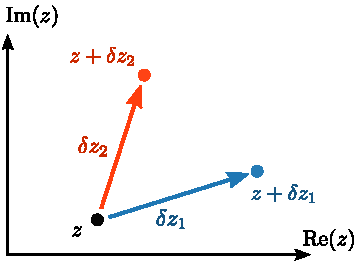
\includegraphics[width=0.37\textwidth]{complex_derivative}
\end{figure}

\clearpage

In principle, we might get different results from the above formula
when we plug in different infinitesimals $\delta z$ and take the limit
$\delta z \rightarrow 0$, even if $f(z)$ is continuous.

\begin{framed}\noindent
  \textit{Example}---Consider the function $f(z) = z^*$.  According to the formula for the complex derivative,
  \begin{align}
    \lim_{\delta z \rightarrow0} \frac{f(z+\delta z) - f(z)}{\delta z} = \lim_{\delta z \rightarrow0} \frac{z^*+\delta z^* - z^*}{\delta z} = \lim_{\delta z \rightarrow0} \frac{\delta z^*}{\delta z}.
  \end{align}
  But if we plug in a real $\delta z$, we get a different result than if we plug in an imaginary $\delta z$:
  \begin{align}
    \begin{aligned}\delta z \in \mathbb{R} \;\; &\Rightarrow \frac{\delta z^*}{\delta z} = 1.\\ \delta z \in i \cdot \mathbb{R} &\Rightarrow \frac{\delta z^*}{\delta z} = -1.\end{aligned}
  \end{align}
\end{framed}

To handle this complication, we regard the complex derivative as
well-defined \textit{only if} the above definition gives the same
answer regardless of the choice of $\mathrm{arg}[\delta z]$. If a
function satisfies this property at a point $z$, we say that it is
\textbf{complex differentiable} at $z$.

The preceding example showed that $f(z) = z^*$ is not complex
differentiable for any $z \in \mathbb{C}$.  The next example shows
that $f(z) = z$ is complex differentiable for all $z \in \mathbb{C}$:

\begin{framed}\noindent
  \textit{Example}---The function $f(z) = z$ is complex differentiable for any $z \in \mathbb{C}$, since
  \begin{align}
    \lim_{\delta z \rightarrow0} \frac{f(z+\delta z) - f(z)}{\delta z} = \lim_{\delta z \rightarrow0} \frac{z+\delta z - z}{\delta z} = \lim_{\delta z \rightarrow0} \frac{\delta z}{\delta z} = 1.
  \end{align}
  The result doesn't depend on $\mathrm{arg}[\delta z]$ because the
  derivative formula simplifies to the fraction $\delta z / \delta z$,
  which is equal to 1 for any $|\delta z| > 0$. Note that we simplify
  the fraction to 1 \textit{before} taking the limit $\delta z
  \rightarrow 0$. We can't take the limit first, because $0/0$ is
  undefined (see Section 1.1.1).
\end{framed}

\subsection{Analytic functions}
\label{analytic-functions}

If a function $f(z)$ is complex differentiable for all $z$ in some
domain $D\subset \mathbb{C}$, then $f(z)$ is said to be
\textbf{analytic} in $D$.

The concepts of analyticity and complex differentiability are closely
related. It's mainly a matter of terminology: we speak of a function
being complex differentiable \textit{at a given point}, and we speak
of a function being analytic \textit{in a given domain}.

\begin{framed}\noindent
  \textit{Example}---As shown in the preceding section, $f(z) = z$ is
  complex-differentiable for any point $z \in \mathbb{C}$.  Thence,
  $f(z) = z$ is analytic in $\mathbb{C}$.
\end{framed}

A function's domain of analyticity is often described spatially, in
terms of the complex plane.  For example, we might say that a function
is analytic ``everywhere in the complex plane'', which means the
entire domain $\mathbb{C}$.  Or we might say that a function is
analytic ``in the upper half of the complex plane'', meaning for all
$z$ such that $\mathrm{Im}(z) > 0$.

\subsubsection{Common analytic functions}
\label{common-analytic-functions}

There is an important class of functions which are analytic over the
entire complex plane, or most of the complex plane.  These are
functions that (i) are expressed in terms of simple algebraic formulas
involving $z$, and (ii) do not contain $z^*$ in the formula.

For example, we have seen that the function $f(z) = z$ is analytic in
$\mathbb{C}$.  Likewise, $f(z) = \alpha z + \beta$, where $\alpha,
\beta$ are complex constants, is analytic everywhere in
$\mathbb{C}$. This can be proven in a similar fashion:
\begin{align}
  f'(z) &= \lim_{\delta z\rightarrow 0} \frac{[\alpha\,(z+\delta z) + \beta] - [\alpha z + \beta]}{\delta z} \\
  &= \lim_{\delta z\rightarrow 0} \frac{\alpha \delta z}{\delta z} \\
  &= \alpha.
\end{align}
We can also show that $f(z) = z^n$, with $n \in \mathbb{N}$, is
analytic everywhere in $\mathbb{C}$:
\begin{align}
  f'(z) &= \lim_{\delta z\rightarrow 0} \frac{(z+\delta z)^n - z^n}{\delta z} \\
  &= \lim_{\delta z\rightarrow 0} \frac{(z^n + n z^{n-1} \delta z + \cdots) - z^n}{\delta z} \\
  &= n z^{n-1}.
\end{align}
Note that these derivatives have exactly the same algebraic formulas
as the corresponding real derivatives. This is no coincidence: to
derive the complex derivatives, we take the same series of algebra
steps used in deriving the real derivatives.

It should thus be evident that any complex polynomial is analytic
everywhere in $\mathbb{C}$. Likewise, functions defined in terms of
power series, including the complex exponential and complex sine and
cosine, are analytic everywhere in $\mathbb{C}$. Functions involving
reciprocals (negative integer powers), such as $f(z) = z^{-1}$ or
$f(z) = z^{-2}$, are analytic everywhere \textit{except} at points
where $f(z)$ becomes singular (i.e., the denominator goes to zero); we
will prove this rigorously in
Section~\ref{consequences-of-the-cauchy-riemann-equations}.

More generally, whenever a function involves $z$ in some combination
of integer polynomials, reciprocals, or functions with power series
expansions---and does not involve $z^*$ in an irreducible way---then
the function is analytic everywhere except at the singular points.
Moreover, the formula for the complex derivative is the same as the
corresponding formula for real derivatives.

\begin{framed}\noindent
  \textit{Example}---The function
  \begin{align}
    f(z) =
    \frac{1}{\cos(z)}
  \end{align}
  is analytic everywhere in $\mathbb{C}$, except for values of $z$
  such that $\cos(z) = 0$. With a bit of work (try it!), one can show
  that these $z$ occur at isolated points along the real line, at $z =
  (m+1/2)\pi$ where $m \in \mathbb{Z}$, and nowhere else in the
  complex plane. The complex derivative is
  \begin{align}
    f'(z) = \frac{\sin(z)}{[\cos(z)]^2}.
  \end{align}
  The easiest way to prove these statements is to use the
  Cauchy-Riemann equations, which are discussed below.
\end{framed}

One proviso should be kept in mind. For non-integer powers, $z^a$
where $a\notin \mathbb{Z}$, the situation is more complicated because
the operation is multi-valued. We'll postpone the discussion of these
special operations until the discussion on branch points and branch
cuts in Chapter 8.

\subsection{The Cauchy-Riemann equations}
\label{the-cauchy-riemann-equations}

The \textbf{Cauchy-Riemann equations} are a pair of real partial
differential equations that provide an alternative way to understand
complex derivatives. Their importance comes from the following
theorem.
\begin{framed}
  \noindent
  Suppose $f$ is a complex function that can be written as
  \begin{align}
    f(z = x + iy) \;=\; u(x,y) + i v(x,y),
  \end{align}
  where $u(x,y)$ and $v(x,y)$ are real functions of two real inputs.
  Then:

  \begin{itemize}
  \item If $f$ is complex differentiable at a point $z = x + i y$,
    then $u$ and $v$ satisfy
  \begin{align}
    \frac{\partial u}{\partial x} = \frac{\partial v}{\partial y} \;\;\;\mathrm{and}\;\;\; \frac{\partial u}{\partial y} = -\frac{\partial v}{\partial x},
  \end{align}
  at the point $(x,y)$.  These are called the Cauchy-Riemann
  equations.

\item If $u$ and $v$ have continuous first partial derivatives that
  satisfy the Cauchy-Riemann equations at a point $(x,y)$, then $f$ is
  complex differentiable at $z = x + iy$.
  \end{itemize}

\end{framed}

\subsubsection{Proof}\label{proof}

We will now prove half of the theorem: the part stating that $f$ being
complex differentiable implies the Cauchy-Riemann equations.  The
converse is left as an exercise.

Suppose $f$ is complex differentiable at some point $z$.  Then there
exists a derivative
\begin{align}
  f'(z) = \lim_{\delta z \rightarrow 0} \frac{f(z+\delta z) - f(z)}{\delta z},
\end{align}
whose value is independent of the argument that we take for the
infinitesimal $\delta z$.  If we take it to be real, i.e. $\delta z =
\delta x \in \mathbb{R}$, the expression for the derivative can be
written as
\begin{align}
  f'(z) &= \lim_{\delta x \rightarrow 0} \frac{f(x+\delta x + i y) - f(x + i y)}{\delta x} \\
  &= \lim_{\delta x \rightarrow 0} \frac{\left[u(x+\delta x, y) + iv(x+\delta x, y)\right] - \left[u(x, y) + i v(x,y)\right]}{\delta x}\\
  &= \lim_{\delta x \rightarrow 0} \frac{\left[u(x+\delta x, y) - u(x,y)\right] + i \left[v(x+\delta x, y)-v(x,y)\right]}{\delta x} \\
  &= \left[ \lim_{\delta x \rightarrow 0} \frac{u(x+\delta x, y) - u(x,y)}{\delta x}\right] + i \left[ \lim_{\delta x \rightarrow 0} \frac{v(x+\delta x, y) - v(x,y)}{\delta x}\right]
\end{align}
On the last line, the quantities in square brackets are the real
partial derivatives of $u$ and $v$ with respect to $x$. Therefore
those partial derivatives are well-defined, and
\begin{align}
  f'(z) = \frac{\partial u}{\partial x} + i \frac{\partial v}{\partial x}.
\end{align}
On the other hand, we could let the infinitesimal be imaginary, by
setting $\delta z = i \delta y$ where $\delta y \in \mathbb{R}$.  Then
\begin{align}
  f'(z) &= \lim_{\delta y \rightarrow 0} \frac{f(x+ i y + i\delta y) - f(x + i y)}{i\delta y} \\
  &= \lim_{\delta y \rightarrow 0} \frac{\left[u(x, y+\delta y) + iv(x, y+\delta y)\right] - \left[u(x, y) + i v(x,y)\right]}{i\delta y}\\
  &= \lim_{\delta y \rightarrow 0} \frac{\left[u(x, y+\delta y) - u(x,y)\right] + i \left[v(x, y+\delta y)-v(x,y)\right]}{i\delta y} \\
  & = -i\frac{\partial u}{\partial y} + \frac{\partial v}{\partial y}
\end{align}
Since $f(z)$ is complex differentiable, these two ways of calculating
$f'(z)$ must give the same result:
\begin{align}
  \frac{\partial u}{\partial x} + i \frac{\partial v}{\partial x} = -i\frac{\partial u}{\partial y} + \frac{\partial v}{\partial y}.
\end{align}
Since $u$ and $v$ are real functions, we can take the real and imaginary parts of the above equation separately.  This yields the Cauchy-Riemann equations,
\begin{align}
  \frac{\partial u}{\partial x} = \frac{\partial v}{\partial y}, \;\;\; \frac{\partial v}{\partial x} = -\frac{\partial u}{\partial y}.
\end{align}
As a corollary, the complex derivative of $f(z)$ can be expressed as:
\begin{align}
  \mathrm{Re}\left[f'(z)\right] &= \frac{\partial u}{\partial x} = \frac{\partial v}{\partial y} \\
  \mathrm{Im}\left[f'(z)\right] &= \frac{\partial v}{\partial x} = -\frac{\partial u}{\partial y}.
\end{align}

\subsubsection{Interpretation of the Cauchy-Rieman equations}
\label{interpretation-of-the-cauchy-riemann-equations}

The basic message of the Cauchy-Riemann equations is that when dealing
with analytic functions, the real and imaginary parts cannot be
regarded as independent quantities, but are closely intertwined.
There are two complementary ways to think about this:

\begin{itemize}
\item For an analytic function $f(z)$, the real and imaginary parts of
  the input $z$ do not independently affect the output value.  If I
  tell you how the function varies in the $x$ direction, by giving you
  $\partial u/\partial x$ and $\partial v/\partial x$, then you can
  work out how the function varies in the $y$ direction, by using the
  Cauchy-Riemann equations to find $\partial u/\partial y$ and
  $\partial v/\partial y$.

\item For the complex outputs of $f(z)$, the real and imaginary parts
  cannot be regarded as independent.  If I tell you how the real part
  of the output varies, by giving you $\partial u/\partial x$ and
  $\partial u/\partial y$, then you can work out how the imaginary
  part of the output varies, by using the Cauchy-Riemann equations to
  find $\partial v/\partial x$ and $\partial v/\partial y$.
\end{itemize}

\noindent
These constraints have profound implications for the mathematical
discipline of complex analysis, one of the most important being
Cauchy's integral theorem, which we will encounter when studying
contour integration in Chapter 9.

\subsubsection{Consequences of the Cauchy-Rieman equations}
\label{consequences-of-the-cauchy-riemann-equations}

Often, the easiest way to prove that a function is analytic in a given
domain is to prove that the Cauchy-Riemann equations are satisfied.

\begin{framed}\noindent
  \textit{Example}---We can use the Cauchy-Riemann equations to prove
  that the function
  \begin{align}
    f(z)=1/z
  \end{align}
  is analytic everywhere, except at $z = 0$.  Let us write the function as
  \begin{align}
    f(x+iy) = \frac{1}{x+iy} = \frac{x-iy}{x^2+y^2}.
  \end{align}
  Hence the real and imaginary component functions are
  \begin{align}
    u(x,y) = \frac{x}{x^2+y^2}, \;\;v(x,y) = - \frac{y}{x^2+y^2}.
  \end{align}
  Except at $x = y = 0$, these functions are differentiable and their
  partial derivatives satisfy the Cauchy-Riemann equations:
  \begin{align}
    \frac{\partial u}{\partial x} &= \frac{-x^2+y^2}{(x^2+y^2)^2} \;= \;\;\;\frac{\partial v}{\partial y} \\ \frac{\partial v}{\partial x} &= \; \frac{2xy}{(x^2+y^2)^2} = -\frac{\partial u}{\partial y}.
  \end{align}
\end{framed}

Moreover, we can use the Cauchy-Riemann equations to prove the
following general facts about analytic functions:

\begin{itemize}
\item \textit{Compositions of analytic functions are analytic}.  If
  $f(z)$ is analytic in $D \subset \mathbb{C}$ and $g(z)$ is analytic
  in the range of $f$, then $g(f(z))$ is analytic in $D$.

\item \textit{Reciprocals of analytic functions are analytic, except
  at singularities}. If $f(z)$ is analytic in $D \subset \mathbb{C}$,
  then $1/f(z)$ is analytic everywhere in $D$ except where $f(z) = 0$.
\end{itemize}

\noindent
The proofs for these can be obtained via the Cauchy-Riemann equations,
and are left as exercises.


\subsection{Exercises}
\label{exercises}

\begin{enumerate}
\item
  For each of the following functions $f(z)$, find the real and
  imaginary component functions $u(x,y)$ and $v(x,y)$, and hence
  verify whether they satisfy the Cauchy-Riemann equations.

  \begin{enumerate}[(a)]
  \item $f(z) = z$
  \item $f(z) = z^2$
  \item $f(z) = |z|$
  \item $f(z) = |z|^2$
  \item $f(z) = \exp(z)$
  \item $f(z) = \cos(z)$
  \item $f(z) = 1/z$
  \end{enumerate}

\item
  Suppose a function $f(z)$ is well-defined and obeys the
  Cauchy-Riemann equations at a point $z$, and the partial derivatives
  in the Cauchy-Riemann equations are continuous at that point. Show
  that the function is complex differentiable at that point. Hint:
  consider an arbitary displacement
  $\Delta z = \Delta x + i \Delta y$.

\item
  Prove that products of analytic functions are analytic: if $f(z)$
  and $g(z)$ are analytic in $D \subset \mathbb{C}$, then
  $f(z) g(z)$ is analytic in $D$.
  \hfill{\scriptsize [solution~available]}

\item
  Prove that compositions of analytic functions are analytic: if
  $f(z)$ is analytic in $D \subset \mathbb{C}$ and $g(z)$ is
  analytic in the range of $f$, then $g(f(z))$ is analytic in $D$.

\item
  Prove that reciprocals of analytic functions are analytic away from
  poles: if $f(z)$ is analytic in $D \subset \mathbb{C}$, then
  $1/f(z)$ is analytic everywhere in $D$ except where $f(z) = 0$.

\item
  Show that if $f(z = x + iy) = u(x,y) + i v(x,y)$ satisfies the
  Cauchy-Riemann equations, then the real functions $u$ and $v$ each
  obey Laplace's equation:
  \begin{equation}
    \frac{\partial^2 u}{\partial x^2} + \frac{\partial^2u}{\partial y^2} = \frac{\partial^2 v}{\partial x^2} + \frac{\partial^2 v}{\partial y^2} = 0.
  \end{equation}
  (Such functions are called ``harmonic functions''.)

\item
  We can write the real and imaginary parts of a function in terms of
  polar coordinates: $f(z) = u(r,\theta) + i v(r,\theta)$, where $z =
  re^{i\theta}$.  Show that the Cauchy-Riemann equations can be
  re-written in polar form as
  \begin{equation}
    \frac{\partial u}{\partial r} =  \frac{1}{r} \frac{\partial v}{\partial \theta}, \quad \frac{\partial v}{\partial r} =  - \frac{1}{r}\,  \frac{\partial u}{\partial \theta}.
  \end{equation}
\end{enumerate}


\end{document}
